One of the many feelings that flourish during the use of a VR is the feeling of presence. This feeling, inside the virtuality context, is when someone feels drawn into a VE and starts to occupy the VE instead of the real one \cite{cummings2016immersive}.

\citeonline{jicol2021effects} explores this feeling in its work. The authors aim to correlate the feeling of presence with one's agency (which is the self-perception that the user is in control of a situation or some actions \cite{farrer2002experiencing}) and emotion, both of these in a VE context. Besides assessing this correlation, the author also did a structural equation model (SEM) based on their findings. The author did this by creating two different VE, one that would trigger happy emotions, and another that would trigger fear. For each VE there were two different variations of it, one that the user could interact with its elements and another that it could not. So at the end, four different VE were designed as the Figures \ref{fig:happy_without} to \ref{fig:fear_with} show.

\begin{figure}[!h] 
    \begin{subfigure}{0.45\textwidth}
    \centering
    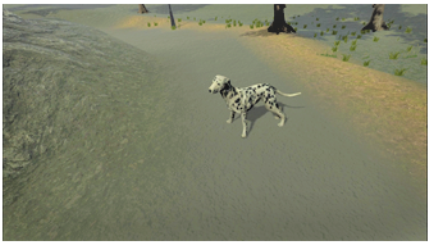
\includegraphics[width=\textwidth]{Revisao/Emotion Presence/Scene Happy No.png} 
    \caption{Without agency.} 
    \label{fig:happy_without}
  \end{subfigure}
  \hfill
  \begin{subfigure}{0.45\textwidth}
    \centering
    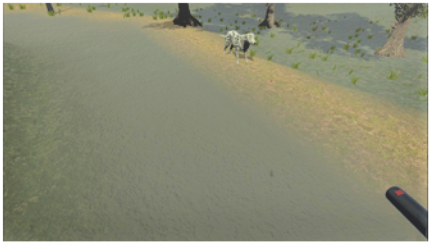
\includegraphics[width=\textwidth]{Revisao/Emotion Presence/Scene Happy Yes.png}
    \caption{With agency.} 
    \label{fig:happy_with}
  \end{subfigure}
\caption{Happy environment \cite{jicol2021effects}.} 
\label{fig:happy_environment}
\end{figure}

\begin{figure}[!h] 
    \begin{subfigure}{0.45\textwidth}
    \centering
    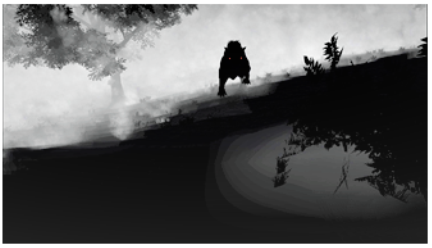
\includegraphics[width=\textwidth]{Revisao/Emotion Presence/Scene Fear No.png}
    \caption{Without agency.} 
    \label{fig:fear_without}
  \end{subfigure}
  \hfill
  \begin{subfigure}{0.45\textwidth}
    \centering
    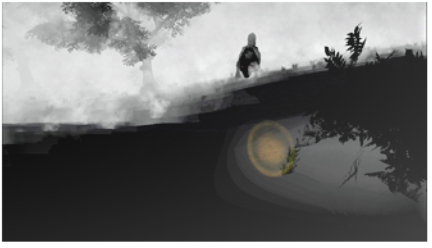
\includegraphics[width=\textwidth]{Revisao/Emotion Presence/Scene Fear Yes.png}
    \caption{With agency.} 
    \label{fig:fear_with}
  \end{subfigure}
\caption{Fear environment \cite{jicol2021effects}.} 
\label{fig:fear_environment}
\end{figure}

This experiment had 121 participants and they were randomly assigned to one of the four VE. Participants with a neurological disease, fear of dogs, psychological or emotional issues, epilepsy or use of the medical device were excluded.

The authors had three hypotheses about their experiment:
\begin{enumerate}
    \item The intensity of the dominant emotion in each VE will correlate positively with the presence
    \item Presence will be significantly higher in environments where participants have agency
    \item Agency will moderate the effect of the emotion on the presence
\end{enumerate}

The first hypothesis was confirmed. No matter if the feeling is positive (happiness) or negative (fear), the users did feel a stronger presence when the positive or negative feelings were more intense.

The second hypothesis was partially correct. In the VE that provoked fear, agency did make a difference and induced a higher feeling of presence, whilst in the VE that provoked happiness, agency did not affect the presence. The same could be said about the third hypothesis.

This is an important work for its findings on the user's presence feeling. Inside a VE, users that have a direct interaction inside it do find a bigger feeling of presence. This is important for this master's thesis experiment. It is possible that, if the participant did not feel "present" inside the VE, the gathered data could be less sensitive to the experiment's goals.

This experiment did not assess directly the feeling of presence, but the feeling of presence inside a VE with BVI users could be a suggestion for future works or even a base study.